\documentclass[12pt, a4paper]{article}

\usepackage{fancyhdr}
\usepackage{extramarks}
\usepackage{amsmath}
\usepackage{amsthm}
\usepackage{amsfonts}  
\usepackage{tikz}
\usepackage{lipsum}
\usepackage[plain]{algorithm}
\usepackage{algpseudocode}
\usepackage{geometry}
\usepackage{graphicx}
\usepackage{subfigure}
\usepackage{setspace}
\usepackage{xcolor}
\usepackage{mathrsfs}
\usepackage{bm}
\usepackage{booktabs}
\usepackage{url}
\usepackage{cite}
\usepackage{gauss}
%\usepackage{bbold}
\usepackage[all]{xy}

\newcommand{\HRule}{\rule{\linewidth}{0.5mm}}
\newcommand{\U}{\ensuremath{\mathrm}}
\newcommand{\celsius}{\ensuremath{^{\circ}\mathrm{C}}}
\newcommand{\dst}{\ensuremath{^{\U{st}}}}
\newcommand{\dnd}{\ensuremath{^{\U{nd}}}}
\newcommand{\drd}{\ensuremath{^{\U{rd}}}}
\newcommand{\dth}{\ensuremath{^{\U{th}}}}
\renewcommand{\mod}{\ \U{mod}\ }
\newcommand{\red}[1]{\textcolor[rgb]{1,0,0}{#1}}

\newcommand{\C}{\mathbb{C}} \newcommand{\F}{\mathbb{F}} \newcommand{\R}{\mathbb{R}} \newcommand{\Q}{\mathbb{Q}}
\newcommand{\N}{\mathbb{N}}

\newtheorem{theorem}{Theorem}
\newtheorem{lemma}{Lemma}

\usetikzlibrary{automata,positioning}
\geometry{left=2.0cm, right=2.0cm, top=2.5cm, bottom=2.5cm}

\pagestyle{fancy}
\lhead{\hmwkClass}
\lfoot{\lastxmark}
\cfoot{\thepage}

\newcommand{\hmwkClass}{VE401}

\setlength{\abovecaptionskip}{0pt}
\setlength{\belowcaptionskip}{10pt}

\begin{document}

\renewcommand\arraystretch{1.5}
\setlength\parskip{.1\baselineskip}

\begin{titlepage}
  \begin{center}
  
\includegraphics[width=0.7\textwidth]{./logo}\\
  \HRule\\[3cm]

  {\Huge\bfseries VE401 Probabilistic Methods in Eng.\\[0.5cm]Solution Manual for RC 4}\\[2cm]
  
  {\large Chen Xiwen}
  \\[1cm]
  {\large \today}
  \vfill

  \textbf{\small University of Michigan--Shanghai Jiao Tong University Joint Institute}
  \end{center}
\end{titlepage}


\newpage

\begin{spacing}{1.1}

%==================================================================================

\section*{Assignment 3.4}

A mathematics textbook has 200 pages on which typographical errors in the equations could occur. Suppose there are in fact five errors randomly dispersed among these 200 pages.
\begin{enumerate}
	\item What is the probability that a random sample of 50 pages will contain at least one error?
	\item How large must the random sample be to assure that at least three errors will be found with 90\% probability? (You may use a normal approximation to the binomial distribution.)
\end{enumerate}
\textbf{\underline{Solution}.}
\begin{enumerate}
	\item The problem is to randomly place the five errors in 200 pages, and each error has the same probability of being placed among the sampled pages.
	\begin{align*}
	P[\U{at\ least\ 1\ error\ in\ 50\ pages}] & = 1 - P[\U{0\ error\ in\ 50\ pages}] \\
	& = 1 - \left(\frac{200-50}{200} \right)^5 \\
	& = 76.27\%.
	\end{align*}
	\item Let the sample size be $k$. The number of selected errors follows a binomial distribution with
	\begin{align*}
	p = \frac{k}{200}, \qquad n = 5,
	\end{align*}
	and thus the mean and standard deviation are given by
	\begin{align*}
	\mu = 5p = \frac{k}{40}, \qquad \sigma = \sqrt{5p(1-p)} = \sqrt{\frac{k}{40}\left(1 - \frac{k}{200} \right)}.
	\end{align*}
	Let $X$ be the number of errors in the sample. Then
	\begin{align*}
	P[X\geq 3] \geq 90\% \quad\Rightarrow\quad P[Y\geq 2.5] \geq 90\%,
	\end{align*}
	where $Y$ follows normal distribution. Transforming to standard normal variable $Z$, we have
	\begin{align*}
	P\left[Z\geq \frac{2.5-\mu}{\sigma} \right]\geq 0.9 \quad\Rightarrow\quad F\left[\frac{2.5-\mu}{\sigma} \right] \leq 0.1 \quad\Rightarrow \quad \frac{2.5-\mu}{\sigma} \leq -1.28,
	\end{align*}
	which gives $k\geq 150$.\\
	\textbf{\underline{Note}.} Some of you may have noticed that the requirements for ``good approximation'' specified in lecture slides are not satisfied. However, if we calculate using $p = 0.75$ and $n = 5$ for binomial distribution,
	\begin{align*}
	P[X\geq 3] = \mathtt{1 - CDF[BinomialDistribution[5, 0.75], 2]} = 0.896484,
	\end{align*}
	which is quite close to 90\%. This posterior validation shows the approximation is reasonable.
\end{enumerate}
\textbf{\underline{About half-unit correction}.} If $X$ follows a binomial distribution with parameters $n$ and $p$, and $Y$ follows a normal distribution with mean $\mu = np$ and variance $\sigma^2 = np(1-p)$. Recall normal approximation to binomial distribution,
\begin{align*}
P[X\leq \red{y}] = \sum_{x=0}^y \binom{n}{x} p^x(1-p)^{n-x} \approx \Phi\left(\frac{\red{y+1/2}-np}{\sqrt{np(1-p)}} \right),
\end{align*}
where $\Phi$ is the cumulative distribution function for the standard normal distribution. Define
\begin{align*}
F(\red{x}) := \Phi\left(\frac{\red{x}-np}{\sqrt{np(1-p)}} \right).
\end{align*}
Then the approximation is simply $P[X\leq y] \approx F(y+1/2)$. We would like to approximate the cumulative distribution of $X$ using the cumulative distribution of $Y$ (denoted as $\Phi$). Consider the following cases. What should be the corresponding approximation? \\
~\\
\begin{minipage}{0.3\linewidth}
	\begin{enumerate}
		\item $P[X \geq x_1]$:
		\begin{enumerate}
			\item $1 - F(x_1 + 0.5)$
			\item $1 - F(x_1 - 0.5)$
		\end{enumerate}
		\item $P[X > x_1]$:
		\begin{enumerate}
			\item $1 - F(x_1 + 0.5)$
			\item $1 - F(x_1 - 0.5)$
		\end{enumerate}
		\item $P[X \leq x_2]$:
		\begin{enumerate}
			\item $F(x_2 + 0.5)$
			\item $F(x_2 - 0.5)$
		\end{enumerate}
		\item $P[X < x_2]$:
		\begin{enumerate}
			\item $F(x_2 + 0.5)$
			\item $F(x_2 - 0.5)$
		\end{enumerate}
	\end{enumerate}
\end{minipage}
\begin{minipage}{0.7\linewidth}
	\centering
	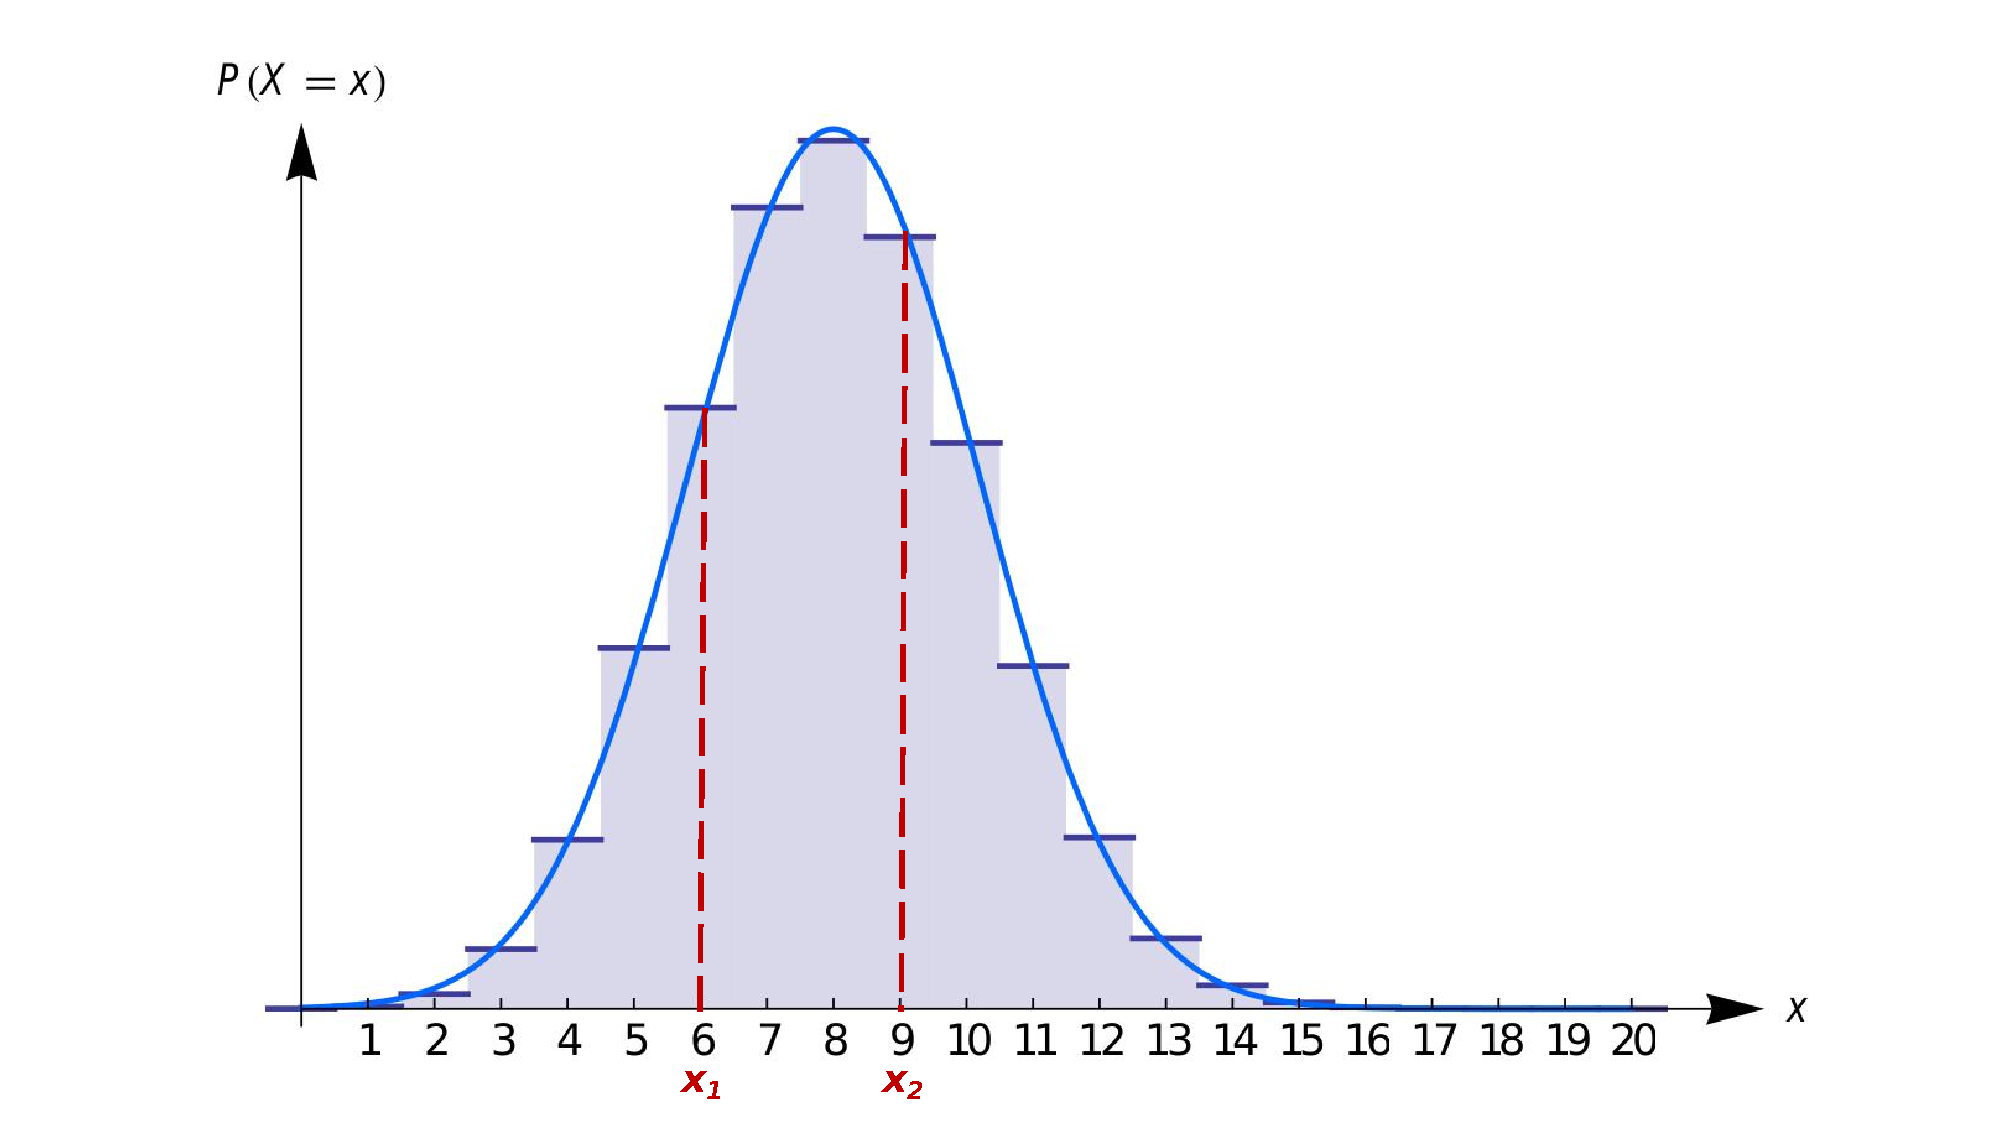
\includegraphics[width=\linewidth]{./images/s4fig1.pdf}
\end{minipage}\\
~\\
~\\
\fbox{
	\emph{Answer}: 1. (b),~~~~ 2. (a),~~~~ 3. (a),~~~~ 4. (b).
} \\
~\\
There are two ways that we can memorize it.
\begin{itemize}
	\item We are approximating the integral of binomial density function. According to the figure, if we want $P[X \leq x]$, then we are calculating the area summing up to the right of $x$. Similarly, if we want $P[X < x]$, we are summing up to the left of $x$.
	\item The original binomial approximation gives
	\begin{align*}
	P[X\leq x] \approx F(x + 1/2),
	\end{align*}
	which means that
	\begin{align*}
	P[X < x] = P[X\leq x - 1] \approx F(x - 1 + 1/2) = F(x - 1/2).
	\end{align*}
\end{itemize}
With this in mind, whenever we want to calculate $P[X\geq x]$ or $P[X > x]$, we rewrite as
\begin{align*}
P[X \geq x] = 1 - P[X < x], \qquad P[X > x] = 1 - P[X\leq x],
\end{align*}
which falls in to the cases discussed above.


\section*{Assignment 3.10}

Let $X = (X_1, X_2)$ be a random vector. Then we define the expectation vector and the variance-covariance matrix as follows.
\begin{align*}
\U{E}[X] := \begin{pmatrix}
\U{E}[X_1] \\ \U{E}[X_2]
\end{pmatrix}, \qquad \U{Var}\ X := \begin{pmatrix}
\U{Var}[X_1] & \U{Cov}(X_1, X_2) \\
\U{Cov}(X_2, X_1) & \U{Var}\ X_2
\end{pmatrix}.
\end{align*}
Let $A$ be a constant $2\times 2$ matrix and $Y = (Y_1, Y_2) = AX$.
\begin{enumerate}
	\item Show that $\U{E}[AX] = A\U{E}[X]$.
	\item Show that $\U{Var}(AX) = A(\U{Var}\ X)A^T$.
	\item Suppose $X_1$ and $X_2$ follow independent normal distributions with mean $\mu_1$ and $\mu_2$ and variances $\sigma_1^2$ and $\sigma_2^2$, respectively. Show that the joint density is given by
	\begin{align*}
	f_X(x) = f_X(x_1, x_2) = \frac{1}{2\pi \sqrt{\det\Sigma_X}} e^{-\frac{1}{2}\langle x - \mu_X, \Sigma_X^{-1}(x - \mu_X) \rangle}
	\end{align*}
	where $\mu_X = (\mu_1, \mu_2)$ and $\Sigma_X = \U{diag}(\sigma_1^2, \sigma_2^2)$ is the $2\times 2$ matrix with the variances on the diagonal and all other entries vanishing.
	\item  Suppose that $X_1$ and $X_2$ follow independent normal distributions with means $\mu_1, \mu_2\in \R$ and variances $\sigma_1^2, \sigma_2^2 > 0$, respectively. Let $Y = AX$ where $A$ is an invertible $n\times n$ matrix. Show that
	\begin{align}\label{eq:1}
	f_Y(y) = \frac{1}{2\pi\sqrt{|\det \Sigma_Y}|} e^{-\frac{1}{2}\langle y - \mu_Y, \Sigma_Y^{-1}(y-\mu_Y)\rangle}
	\end{align}
	where $\mu_Y = \U{E}[Y]$, $\Sigma_Y = \U{Var}\ Y$ and $\langle \cdot, \cdot\rangle$ denotes the euclidean scalar product in $\R^2$.
	\item Show that Eq. (\ref{eq:1}) can be written as
	\begin{align*}
	f_Y(y_1, y_2) = \frac{1}{2\pi \sigma_{Y_1}\sigma_{Y_2}\sqrt{1-\rho^2}} e^{-\frac{1}{2(1-\rho^2)}\left[\left(\frac{y_1 - \mu_{Y_1}}{\sigma_{Y_1}} \right)^2 - 2\rho\left(\frac{y_1-\mu_{Y_1}}{\sigma_{Y_1}} \right)\left(\frac{y_2 - \mu_{Y_2}}{\sigma_{Y_2}} \right) + \left(\frac{y_2 - \mu_{Y_2}}{\sigma_{Y_2}} \right)^2 \right]}
	\end{align*}
	where $\mu_{Y_i}$ is the mean and $\sigma_{Y_i}^2$ the variance of $Y_i, i = 1, 2$, and $\rho$ is the correlation of $Y_1$ and $Y_2$.
\end{enumerate}
\textbf{\underline{Solution}.}
\begin{enumerate}
	\item Following properties for expectation, we have
	\begin{align*}
	\U{E}[AX] = \U{E}\left[
	\begin{pmatrix}
	a_{11}X_1 + a_{12}X_2 \\ a_{21}X_1 + a_{22}X_2
	\end{pmatrix}
	\right] = \begin{pmatrix}
	a_{11}\U{E}[X_1] + a_{12}\U{E}[X_2] \\
	a_{21}\U{E}[X_1] + a_{22}\U{E}[X_2]
	\end{pmatrix} = A\U{E}[X].
	\end{align*}
	\item By definition, we have
	\begin{align*}
	\U{Var}(AX) & = \U{Var}\begin{pmatrix}
	a_{11}X_1 + a_{12}X_2 \\
	a_{21}X_1 + a_{22}X_2
	\end{pmatrix} \\
	& = \begin{pmatrix}
	\U{Var}(a_{11}X_1 + a_{12}) & \U{Cov}(a_{11}X_1 + a_{12}X_2, a_{21}X_1 + a_{22}X_2) \\
	\U{Cov}(a_{21}X_1 + a_{22}X_2, a_{11}X_1 + a_{12}X_2) & \U{Var}(a_{21}X_1 + a_{22}X_2)
	\end{pmatrix}.
	\end{align*}
	From the properties of variance and covariance, we have
	\begin{align*}
	\U{Var}(a_{11}X_1 + a_{12}X_2) & = a_{11}^2\U{Var}X_1 + a_{12}^2\U{Var}X_2 + 2a_{11}a_{12}\U{Cov}(X_1, X_2), \\
	\U{Var}(a_{21}X_1 + a_{22}X_2) & = a_{21}^2\U{Var}X_1 + a_{22}^2\U{Var}X_2 + 2a_{21}a_{22}\U{Cov}(X_1, X_2),
	\end{align*}
	and
	\begin{align*}
	\U{Cov}(a_{11}X_1 + a_{12}X_2, a_{21}X_1 + a_{22}X_2) & = \U{Cov}(a_{21}X_1 + a_{22}X_2, a_{11}X_1 + a_{12}X_2) \\
	& = a_{11}a_{21}\U{Var}(X_1) + a_{12}a_{22}\U{Var}(X_2) + \\
	& \qquad\qquad\qquad + (a_{11}a_{22} + a_{12}a_{21})\U{Cov}(X_1, X_2).
	\end{align*}
	Therefore,
	\begin{align*}
	A(\U{Var}\ X)A^T & = \begin{pmatrix}
	a_{11} & a_{12} \\
	a_{21} & a_{22}
	\end{pmatrix}\begin{pmatrix}
	a_{11}\U{Var}X_1 + a_{12}\U{Cov}(X_1, X_2) & a_{21}\U{Var}X_1 + a_{22}\U{Cov}(X_1, X_2) \\
	a_{11}\U{Cov}(X_2, X_1) + a_{12}\U{Var}X_2 & a_{21}\U{Cov}(X_1, X_2) + a_{22}\U{Var}X_2
	\end{pmatrix} \\
	& = \U{Var}(AX).
	\end{align*}
	\item We have
	\begin{align*}
	\sqrt{\det \Sigma_X} = \sigma_1\sigma_2, \qquad \Sigma_X^{-1} = \begin{pmatrix}
	1/\sigma_1^2 & 0 \\
	0 & 1/\sigma_2^2
	\end{pmatrix}.
	\end{align*}
	and
	\begin{align*}
	\langle x - \mu_X, \Sigma_X^{-1}(x - \mu_X)\rangle = \frac{(x_1 - \mu_1)^2}{\sigma_1^2} + \frac{(x_2 - \mu_2)^2}{\sigma_2^2}.
	\end{align*}
	Since $X_1$ and $X_2$ are independent, 
	\begin{align*}
	f_X(x) & = f_X(x_1, x_2) = f_{X_1}(x_1)\cdot f_{X_2}(x_2) \\
	& = \frac{1}{2\pi \sigma_1\sigma_2} e^{-\frac{1}{2}\left(\frac{(x_1 - \mu_1)^2}{\sigma_1^2} + \frac{(x_2-\mu_2)^2}{\sigma_2^2} \right)} \\
	& = \frac{1}{2\pi \sqrt{\det \Sigma_X}} e^{-\frac{1}{2}\langle x-\mu_X, \Sigma_X^{-1}(x-\mu_X)\rangle}.
	\end{align*}
	\item Since $Y = AX$, from (1) and (2) we know that
	\begin{align*}
	\mu_Y = \U{E}[AX] = A\mu_X, \qquad \Sigma_Y = A\Sigma_X A^T \quad & \Rightarrow\quad \Sigma_Y^{-1} = (A^T)^{-1}\Sigma_X^{-1}A^{-1}, \\
	& \Rightarrow\quad \det\Sigma_Y = (\det A)^2\det\Sigma_X.
	\end{align*}
	Using transformation of variables,
	\begin{align*}
	f_Y(y) & = f_Y\circ (A^{-1}y) \cdot |\det A^{-1}| \\
	& = \frac{1}{2\pi \sqrt{\det\Sigma_X}} e^{-\frac{1}{2}\langle A^{-1}y - A^{-1}\mu_Y, \Sigma_X^{-1}(A^{-1}y - A^{-1}\mu_Y)\rangle} \cdot \frac{1}{|\det A|} \\
	& = \frac{1}{2\pi \sqrt{\det \Sigma_X \cdot (\det A)^2}} e^{-\frac{1}{2}\langle y - \mu_Y, \Sigma_Y^{-1}(y - \mu_Y)\rangle} \\
	& = \frac{1}{2\pi \sqrt{|\det \Sigma_Y|}} e^{-\frac{1}{2}\langle y - \mu_Y, \Sigma_Y^{-1}(y - \mu_Y)\rangle}.
	\end{align*}
	\item Rewriting $\sqrt{|\det \Sigma_Y|}$ as
	\begin{align*}
	\sqrt{|\det \Sigma_Y|} & = \sqrt{\sigma_{Y_1}^2\sigma_{Y_2}^2 - \U{Cov}^2(Y_1, Y_2)} \\
	& = \sigma_{Y_1}\sigma_{Y_2}\sqrt{1 - \left(\frac{\U{Cov}(Y_1, Y_2)}{\sigma_{Y_1}\sigma_{Y_2}} \right)^2} \\
	& = \sigma_{Y_1}\sigma_{Y_2}\sqrt{1-\rho^2},
	\end{align*}
	and
	\begin{align*}
	\Sigma_Y = \begin{pmatrix}
	\sigma_{Y_1}^2 & \rho\sigma_{Y_1}\sigma_{Y_2} \\
	\rho\sigma_{Y_1}\sigma_{Y_2} & \sigma_{Y_2}^2
	\end{pmatrix} \quad\Rightarrow\quad \Sigma_Y^{-1} = \frac{1}{1-\rho^2}\begin{pmatrix}
	\frac{1}{\sigma_{Y_1}^2} & -\frac{\rho}{\sigma_{Y_1}\sigma_{Y_2}} \\
	-\frac{\rho}{\sigma_{Y_1}\sigma_{Y_2}} & \frac{1}{\sigma_{Y_2}^2}
	\end{pmatrix},
	\end{align*}
	we have
	\begin{align*}
	\langle y-\mu_Y, \Sigma_Y(y-\mu_Y)\rangle & = \frac{1}{1-\rho^2}\langle \begin{pmatrix}
	y_1-\mu_{Y_1} \\ y_2-\mu_{Y_2}
	\end{pmatrix}, \begin{pmatrix}
	\frac{1}{\sigma_{Y_1}^2} & -\frac{\rho}{\sigma_{Y_1}\sigma_{Y_2}} \\
	-\frac{\rho}{\sigma_{Y_1}\sigma_{Y_2}} & \frac{1}{\sigma_{Y_2}^2}
	\end{pmatrix}\rangle \\
	& = \frac{1}{1-\rho^2} \left[\left(\frac{y_1-\mu_{Y_1}}{\sigma_{Y_1}} \right)^2 - 2\rho\left(\frac{y_1-\mu_{Y_1}}{\sigma_{Y_1}} \right)\left(\frac{y_2-\mu_{Y_2}}{\sigma_{Y_2}} \right) + \left(\frac{y_2-\mu_{Y_2}}{\sigma_{Y_2}} \right)^2  \right].
	\end{align*}
	Therefore, Eq. (\ref{eq:1}) can be written as
	\begin{align*}
	f_Y(y_1, y_2) = \frac{1}{2\pi \sigma_{Y_1}\sigma_{Y_2}\sqrt{1-\rho^2}} e^{-\frac{1}{2(1-\rho^2)}\left[\left(\frac{y_1 - \mu_{Y_1}}{\sigma_{Y_1}} \right)^2 - 2\rho\left(\frac{y_1-\mu_{Y_1}}{\sigma_{Y_1}} \right)\left(\frac{y_2 - \mu_{Y_2}}{\sigma_{Y_2}} \right) + \left(\frac{y_2 - \mu_{Y_2}}{\sigma_{Y_2}} \right)^2 \right]}.
	\end{align*}
\end{enumerate}


\section*{Assignment 3.11}

A system consists of two independent components connected in series. The life span (in hours) of the component follows a Weibull distribution with $\alpha = 0.006$ and $\beta = 0.5$; the second has a lifespan in hours follows the exponential distribution with $\beta = 1/25000$.
\begin{enumerate}
	\item Find the reliability of the system at 2500 hours.
	\item Find the probability that the system will fail before 2000 hours.
	\item If the two components are connected in parallel, what is the system reliability at 2500 hours?
\end{enumerate}
\textbf{\underline{Solution}.}
\begin{enumerate}
	\item The reliability function for the two components are given by
	\begin{align*}
	R_1(t) = e^{-\alpha_1 t^{\beta_1}}, \qquad R_2(t) & = 1 - \int_0^t f_{T_2}(x)\U{d}x \\
	& = 1 + e^{-\beta_2 x}\bigg|_0^t = e^{-\beta_2 t}.
	\end{align*}
	Therefore, the reliability of the system at $t = 2500$ is given by
	\begin{align*}
	R(t) = R_1(t)\cdot R_2(t) \quad \Rightarrow\quad R(2500) = 0.7408\times 0.9048 = 0.6703.
	\end{align*}
	\item The probability that the system fail before 2000h is given by
	\begin{align*}
	P[T < 2000] = 1 - R(2000) = 1 - 0.7059 = 0.2941.
	\end{align*}
	\item The reliability at $t = 2500$ for the parallel system is
	\begin{align*}
	R(t) = 1 - (1-R_1(t))(1-R_2(t)) \quad\Rightarrow\quad R(2500) = 0.9753.
	\end{align*}
\end{enumerate}



\section*{Assignment 4.2}

Let $X_1, \ldots, X_n$ be a random sample of size $n$ from a random variable with variance $\sigma^2$. We have seen that the sample variance
\begin{align*}
S_{n-1}^2 := \frac{1}{n-1} \sum_{k=1}^n (X_k - \overline{X})^2
\end{align*}
is an unbiased estimator for $\sigma^2$. It can be shown that
\begin{align}\label{eq:2}
\U{Var}(S_{n-1}^2) = \U{MSE}(S_{n-1}^2) = \frac{1}{n}\left(\U{E}[(X - \overline{X})^4] - \frac{n-3}{n-1}\sigma^4 \right) = \frac{1}{n}\left(\gamma_2 + \frac{2n}{n-1} \right)\sigma^4
\end{align}
where $\gamma_2 := \U{E}[(X - \mu)^4]/\sigma^4 - 3$ is called the \emph{excess kurtosis} of a distribution.
\begin{enumerate}
	\item Show that if $X$ follows a normal distribution with mean $\mu$ and variance $\sigma^2$,
	\begin{align*}
	\U{MSE}(S_{n-1}^2) = \frac{2}{n-1}\sigma^4.
	\end{align*}
	\item For $a > 0$ set
	\begin{align*}
	S_a^2 := \frac{n-1}{a} S_{n-1}^2.
	\end{align*}
	Find $\U{MSE}(S_a^2)$ and show that the mean square error is minimized for
	\begin{align*}
	a = n + 1 + \frac{n-1}{n}\gamma_2.
	\end{align*}
	In the case of a normal distribution with mean $\mu$ and variance $\sigma^2$, show that this reduces to $a = n + 1$.
\end{enumerate}
\textbf{\underline{Solution}.}
\begin{enumerate}
	\item We know that,
	\begin{align*}
	\U{MSE}[S_{n-1}^2] & = \U{Var}[S_{n-1}^2] + \U{bias}^2 = \U{Var}[S_{n-1}^2].
	\end{align*}
	Since $X$ follows a normal distribution,
	\begin{align*}
	\chi_{n-1}^2 = \frac{(n-1)S_{n-1}}{\sigma^2}
	\end{align*}
	follows Chi-squared distribution with $n-1$ degrees of freedom. The variance is
	\begin{align*}
	\U{Var}[\chi_{n-1}^2] = 2(n-1) \quad\Rightarrow\quad \U{Var}[S_{n-1}^2] & = \frac{\sigma^4}{(n-1)^2}\cdot 2(n-1) = \frac{2\sigma^4}{n-1}.
	\end{align*}
	\item By definition, the MSE for $S_a^2$ is given by
	\begin{align*}
	\U{MSE}[S_a^2] & = \U{E}[S_a^4 - 2\sigma^2 S_a^2 + \sigma^4] \\
	& = \U{E}[S_a^4] - 2\sigma^2 \cdot \frac{n-1}{a}\sigma^2 + \sigma^4 \\
	& = \U{E}[S_a^4] + \left(1 - \frac{2(n-1)}{a} \right)\sigma^4.
	\end{align*}
	Using Eq. (\ref{eq:2}) and property for variance, we have
	\begin{align*}
	\U{E}[S_a^4] & = \U{Var}[S_a^2] + \U{E}[S_a^2]^2 \\
	& = \frac{(n-1)^2}{a^2}\U{Var}[S_{n-1}^2] + \frac{(n-1)^2}{a^2}\sigma^4, \\
	\U{MSE}[S_a^4] & = \frac{(n-1)^2}{a^2}\cdot\frac{1}{n}\left(\gamma_2 + \frac{2n}{n-1} \right)\sigma^4 + \frac{(n-1)^2}{a^2}\sigma^4 + \left(1 - \frac{2(n-1)}{a} \right)\sigma^4 \\
	& = \left[x^2\cdot\frac{1}{n}\left(\gamma_2+\frac{2n}{n-1} \right) + x^2 - 2x + 1 \right]\sigma^4 \qquad \left(\U{let\ } x = \frac{n-1}{a}\right) \\
	& = \left[\left(\frac{\gamma_2}{n} + \frac{2}{n-1} + 1\right)x^2 - 2x + 1 \right],
	\end{align*}
	which is maximized when
	\begin{align*}
	x = \frac{1}{\dfrac{\gamma_2}{n} + \dfrac{2}{n-1} + 1} = \frac{n-1}{a}\quad \Rightarrow\quad a = n + 1 + \frac{n-1}{n}\gamma_2.
	\end{align*}
	In case of normal distribution with mean $\mu$ and variance $\sigma^2$, since
	\begin{align*}
	\gamma_2 = \U{E}\left[\frac{(X-\mu)^4}{\sigma^4} \right] - 3 = \U{E}[Z^4] - 3,
	\end{align*}
	where $Z$ follows a standard normal distribution and $\U{E}[Z^4]$ is the 4th moment of it, given by
	\begin{align*}
	\U{E}[Z^4] = \frac{\U{d}^4m_Z(t)}{\U{d}t^4}\bigg|_{t=0} = (t^4 + 6t^2 + 3) e^{\frac{1}{2}t^2}\bigg|_{t=0} = 3,
	\end{align*}
	and thus
	\begin{align*}
	a = n + 1.
	\end{align*}
\end{enumerate}

\section*{Mean and Variance for Estimators}

We know that the mean square error is given by
\begin{align*}
\U{MSE}[\widehat{\theta}] & = \U{E}[(\widehat{\theta} - \theta)^2] \\
& = \U{E}[(\widehat{\theta} - \U{E}[\widehat{\theta}] + \U{E}[\widehat{\theta}] - \theta)^2] \\
& = \U{E}[(\widehat{\theta} - \U{E}[\widehat{\theta}])^2] + \U{E}[2(\widehat{\theta} - \U{E}[\widehat{\theta}])(\U{E}[\widehat{\theta}] - \theta)] + \U{E}[(\U{E}[\widehat{\theta}] - \theta)^2] \\
& = \U{Var}\ \widehat{\theta} + \U{bias}^2.
\end{align*}
MSE is an overall measurement of the quality of the estimator. This means that under the same MSE, estimators with lower bias have a larger variance, and vice versa. This is called the bias-variance trade-off. Therefore, depending on the context, we might prefer a smaller bias or smaller variance.

Here we analyze the mean and variance for unbiased estimators that we have seen in lectures and assignments. For now on, suppose we have sample $X_1, \ldots, X_n$ from a population $X$ with mean $\mu$ and variance $\sigma^2$.

\subsection*{Mean}

The unbiased estimator for mean is given by
\begin{align*}
\widehat{\mu} = \frac{1}{n}\sum_{i=1}^n X_i.
\end{align*}
Then the mean and variance for this estimator are given by
\begin{align*}
\U{E}[\widehat{\mu}] & = \U{E}\left[\frac{1}{n}\sum_{i=1}^n X_i \right] = \frac{1}{n}\sum_{i=1}^n \U{E}[X_i] = \mu, \\
\U{Var}\ \widehat{\mu} & = \U{Var}\left(\frac{1}{n}\sum_{i=1}^n X_i \right) = \sum_{i=1}^n \frac{1}{n^2} \U{Var}\ X_i = \frac{\sigma^2}{n}.
\end{align*}

\subsection*{Variance}

The unbiased estimator for variance is given by
\begin{align*}
\widehat{\sigma^2} = \frac{1}{n-1}\sum_{i=1}^n (X_i - \overline{X})^2.
\end{align*}
Then
\begin{align*}
\U{E}[\widehat{\sigma^2}] & = \frac{1}{n-1} \U{E}\left[\sum_{i=1}^n X_i^2 - 2X_i\overline{X} + \overline{X}^2 \right] \\
& = \frac{1}{n-1} \U{E}\left[\sum_{i=1}^n X_i^2 - n\overline{X}^2 \right] \\
& = \frac{1}{n-1}\left(\sum_{i=1}^n \U{E}[X_i^2] - n\U{E}[\overline{X}^2] \right) \\
& = \frac{1}{n-1}\left(n(\sigma^2 + \mu^2) - n\left(\frac{\sigma^2}{n} + \mu^2 \right) \right) \\
& = \sigma^2.
\end{align*}
For variance of this estimator, we have
\begin{align*}
\U{Var}\ \widehat{\sigma^2} & = \U{Var}\left(\frac{1}{n-1}\sum_{i=1}^n (X_i - \overline{X})^2 \right) \\
& = \U{E}\left[\left(\frac{1}{n-1}\sum_{i=1}^n (X_i - \overline{X})^2 - \sigma^2\right)^2 \right].
\end{align*}
Rewriting sample variance as
\begin{align*}
S^2 & = \frac{1}{n-1} \left(\sum_{i=1}^n X_i^2 - \frac{1}{n}\left(\sum_{i=1}^n X_i \right)^2 \right) \\
& = \frac{1}{n(n-1)} \left((n-1)\sum_{i=1}^n X_i^2 - 2\sum_{i<j}X_iX_j \right) \\
& = \frac{1}{n(n-1)} \sum_{i<j} (X_i - X_j)^2,
\end{align*}
we have
\begin{align*}
\U{E}[(\widehat{\sigma^2} - \sigma^2)^2] & = \U{E}[S^4 - 2\sigma^2S^2 + \sigma^4] \\
& = \U{E}\left[\left(\frac{1}{n(n-1)} \sum_{i<j} (X_i - X_j)^2 \right)^2 \right] - \sigma^4 \\
& = \U{E}\left[\left(\frac{1}{n(n-1)} \sum_{i<j} (X_i - X_j)^2 \right)\left(\frac{1}{n(n-1)} \sum_{p<q} (X_p - X_q)^2 \right) \right] - \sigma^4.
\end{align*}
Expanding the product above, we can have the following cases regarding the values of $i, j$ and $p, q$. Denote the $k$th moment of $X$ as $\U{E}[X^k] = m_k$.
\begin{itemize}
	\item \underline{$i = j, p = q$}.  Since $X_i$ and $X_j$ are independent,
	\begin{align*}
	\U{E}[(X_i-X_j)^4] & = \U{E}[X_i^4 - 4X_i^3X_j + 6X_i^2X_j^2 - 4X_iX_j^3 + X_j^4] \\
	& = 2m_4 - 8m_1m_3 + 6m_2^2.
	\end{align*}
	There are $\dfrac{n(n-1)}{2}$ ways of choosing $i, j$, and thus there are the same number of such terms.
	\item \underline{$|\{i, j\}\cap\{p, q\}| = 1$}. $|\cdot|$ is the cardinality of set. Suppose for now that $j = q$.
	\begin{align*}
	\U{E}[(X_i-X_j)^2(X_p-X_q)^2] & = \U{E}[(X_iX_p-X_iX_q-X_pX_q+X_q^2)^2] \\
	& = \U{E}[X_i^2X_p^2 + X_i^2X_q^2 + X_p^2X_q^2 + X_q^4 -  \\
	& \qquad \qquad \qquad - 2X_i^2X_pX_q - 2X_iX_p^2X_q + 2X_iX_pX_q^2 + \\
	& \qquad \qquad \qquad + 2X_iX_pX_q^2 - 2X_iX_q^3 - 2X_pX_q^3 ] \\
	& = m_4 + 3m_2^2 - 4m_1m_3.
	\end{align*}
	There are $n(n-1)(n-2)$ ways of such terms.
	\item \underline{$i\neq j\neq p\neq q$}. Since the four variables are independent, 
	\begin{align*}
	\U{E}[(X_i-X_j)^2(X_p-X_q)^2] & = \left(\U{E}[(X_i-X_j)^2] \right)^2 \\
	& = \left(\U{E}[X_i^2 - 2X_iX_j + X_j^2] \right)^2 \\
	& = \left(2m_2 - 2m_1^2 \right)^2 \\
	& = 4m_2^2 - 8m_1^2m_2 + 4m_1^4.
	\end{align*}
	There are $\dfrac{n(n-1)(n-2)(n-3)}{4}$ ways of choosing $i, j, p, q$, and thus there are the same number of such terms.
\end{itemize}
Summing up, we have
\begin{align*}
\U{E}[\widehat{\sigma^2}] & = \frac{1}{n^2(n-1)^2}\U{E}\left[\left(\sum_{i<j}(X_i-X_j)^2\right)^2 \right] \\
& = \frac{1}{n}\left(m_4 - 4m_1m_3 - \frac{n-3}{n-1}m_2^2 + \frac{4(2n-3)}{n-1}m_1^2m_2 - \frac{2(2n-3)}{n-1}m_1^4 \right),
\end{align*}
which coincides with what is given in Assignment 4.2, where 
\begin{align*}
\frac{1}{n}\left(\gamma_2 + \frac{2n}{n-1}\right)\sigma^4 & = \frac{1}{n}\left(\U{E}[(X-\mu)^4] - \frac{n-3}{n-1}(m_2-m_1^2)^2 \right) \\
& = \frac{1}{n}\left(\U{E}[X^4 - 4X^3\mu + 6X^2\mu^2 - 4X\mu^3 + \mu^4] - \frac{n-3}{n-1}(m_2-m_1^2)^2 \right) \\
& = \frac{1}{n}\left(m_4 - 4m_1m_3 + 6m_1^2m_2 - 3m_1^4 - \frac{n-3}{n-1}(m_1^4 - 2m_1^2m_2 + m_2^2) \right) \\
& = \frac{1}{n}\left(m_4 - 4m_1m_3 + \frac{8n-12}{n-1}m_1^2m_2 - \frac{n-3}{n-1}m_2^2 - \frac{4n-6}{n-1}m_1^4 \right).
\end{align*}


  
\end{spacing}
\end{document}
